\chapter{A Path Towards Calibration of the OVRO-LWA}
\label{chapter2}

\section{Design and Construction of the OVRO-LWA}

\begin{bibunit}

\begin{figure}[t]
    \centering
    \begin{tabular}{cc}
        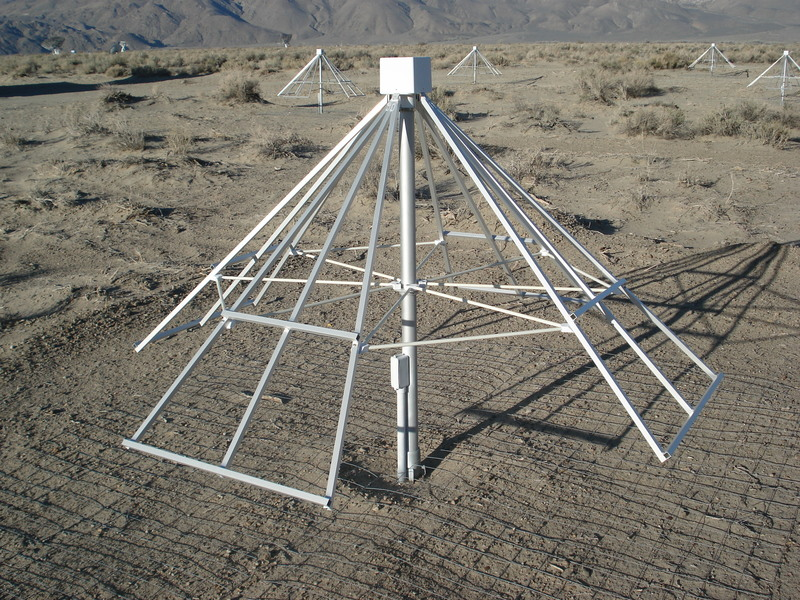
\includegraphics[height=4cm]{figures/chapter2/lwa-antenna} &
        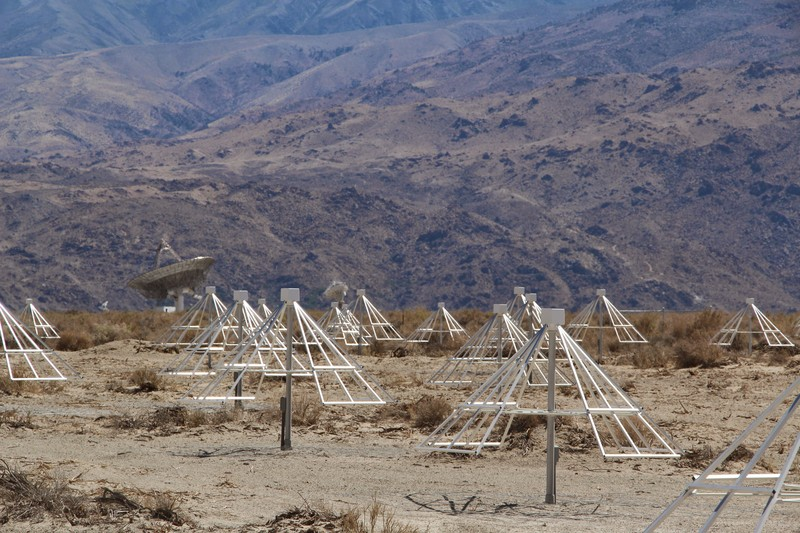
\includegraphics[height=4cm]{figures/chapter2/ovro-lwa} \\
        (a) & (b) \\
    \end{tabular}
    \caption{
        (a) A picture of an OVRO-LWA antenna.
        (b) A view of the OVRO-LWA with the Sierra Mountains in the background.
    }
    \label{fig:ovro-lwa-pictures}
\end{figure}

\begin{figure}[t]
    \centering
    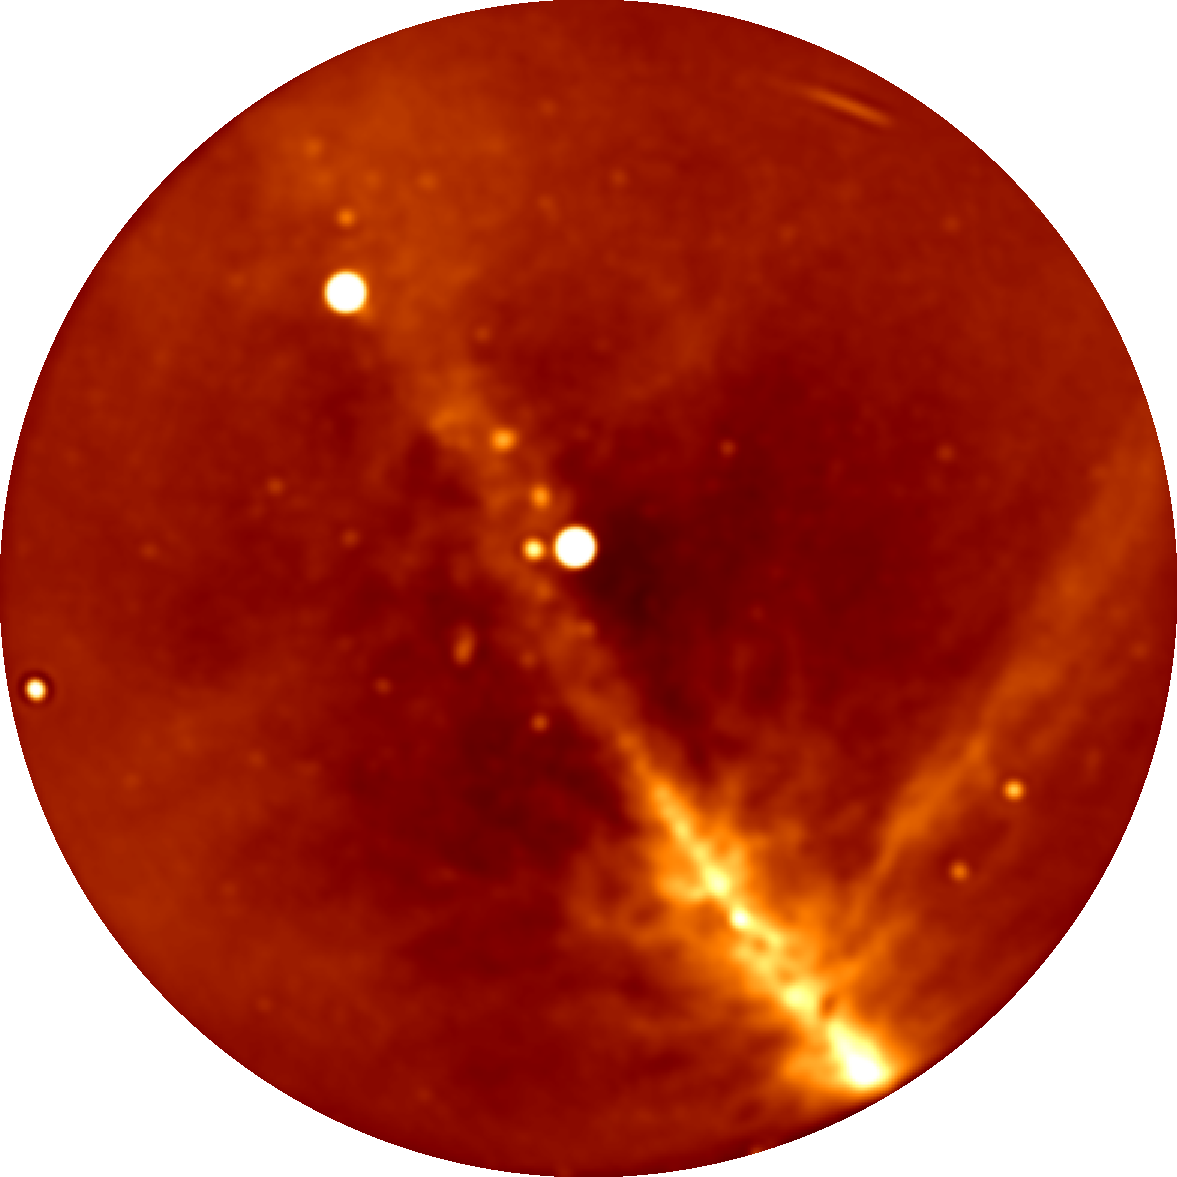
\includegraphics[width=\textwidth]{figures/chapter2/ovro-lwa-core-image}
    \caption{
        Snapshot dirty image of the sky captured with the OVRO-LWA using just the antennas located
        in the core of the array. Cyg~A and Cas~A have been peeled and restored with model sources.
    }
    \label{fig:core-snapshot-image}
\end{figure}

\begin{figure}[t]
    \centering
    \includegraphics[width=\textwidth]{figures/chapter2/ovro-lwa-expansion-image/ovro-lwa-expansion-image}
    \caption{
        Snapshot image of the sky captured with the OVRO-LWA using the new long-baseline antennas.
    }
    \label{fig:expansion-snapshot-image}
\end{figure}

The Owens Valley Radio Observatory Long Wavelength Array (OVRO-LWA) is a new low-frequency radio
interferometer constructed during the course of this thesis (see
Figure~\ref{fig:ovro-lwa-pictures}). In its current iteration, it is composed of 288
dual-polarization dipole antennas with a bandpass covering 27 to 85~MHz (wavelengths between 3.5 and
11~m). 251 antennas are located with a 200~m diameter core in a pseudo-random configuration
optimized for minimum sidelobes in snapshot imaging. 32 additional antennas are located at distances
up to 1.5~km from the core of the array. At 85~MHz, the OVRO-LWA can therefore achieve an angular
resolution of 8\arcmin. Figures~\ref{fig:core-snapshot-image} and \ref{fig:expansion-snapshot-image}
illustrate the improvement in angular resolution associated with using these long baselines.

The OVRO-LWA hosts the LEDA correlator \citep{2015JAI.....450003K}, which performs full
cross-correlation of 512 input signals.

Paragraph on antenna

Paragraph on receivers

Paragraph on correlator


During observations, data is streamed from the LEDA correlator to the All-Sky Transient Monitor
(ASTM), which houses the compute nodes used for post-processing, imaging, and the analysis completed
in this thesis.

ASTM is composed of 10 identical nodes.\todo{Fill out specs once ASTM is back online....}


There are two complementary software pipelines that service the scientific goals of the OVRO-LWA:
\begin{enumerate}
    \item A widefield snapshot imaging pipeline that images the entire visible hemisphere every
        13\,s.
    \item A novel approach specialized for drift-scanning interferometers that can image the entire
        sky (above a limiting declination) in a single synthesis imaging step.
\end{enumerate}
The latter pipeline will be discussed in considerable depth in Chapters~\ref{chapter3} and
\ref{chapter4}.

\section{Calibration of a Low-Frequency Interferometer}

Gain calibration amounts to determining the optimal set of Jones matrices $G_i$ for each antenna $i$
such that
\begin{align}
    \b V_{ij, \text{measured}} &= \b G_i \, \b V_{ij, \text{model}} \, \b G_j^*
        + \b N_{ij} \\
    \begin{pmatrix}
        V_{ij, \text{measured}}^{xx} & V_{ij, \text{measured}}^{xy} \\
        V_{ij, \text{measured}}^{yx} & V_{ij, \text{measured}}^{yy} \\
    \end{pmatrix} &=
    \begin{pmatrix}
        g_{i}^{xx} & g_{i}^{xy} \\
        g_{i}^{yx} & g_{i}^{yy} \\
    \end{pmatrix}
    \begin{pmatrix}
        V_{ij, \text{model}}^{xx} & V_{ij, \text{model}}^{xy} \\
        V_{ij, \text{model}}^{yx} & V_{ij, \text{model}}^{yy} \\
    \end{pmatrix}
    \begin{pmatrix}
        g_{j}^{xx} & g_{j}^{xy} \\
        g_{j}^{yx} & g_{j}^{yy} \\
    \end{pmatrix}^* +
    \begin{pmatrix}
        n_{j}^{xx} & n_{j}^{xy} \\
        n_{j}^{yx} & n_{j}^{yy} \\
    \end{pmatrix}\,,
\end{align}
where $\b V_{ij,\text{measured}}$ is the Jones matrix of measured visibilities on the baseline
$i-j$, $\b V_{ij,\text{model}}$ is the Jones matrix of model visibilities (i.e., ideally what would
have been measured if the antenna and receiver did not impart any additional gain or phase), and $\b
N_{ij}$ is additional noise.

A typical calibration strategy using the Very Large Array (VLA) involves periodically pointing at a
known compact point source. For a compact point source at the phase center, the phase of all
visibilities should be zero, and the amplitude is given by the known flux (and if necessary, the
polarization) of the source.

The OVRO-LWA is capable of imaging the entire hemisphere in a snapshot image. This brings its own
unique calibration challenges because it is currently impossible to isolate a single compact point source
within the field of view of the interferometer.\footnote{
    Gated pulsar observations could, in principle, achieve this isolation. This capability is a key
    development area for the OVRO-LWA.
}
Due to the wide field of view, determining an accurate gain calibration relies on a detailed sky
and antenna beam model. Mistakes or omissions in the sky model can, for example, generate artificial
ripples in the bandpass calibration that will impact the interferometer's ability to cleanly
separate foreground emission from cosmological 21~cm emission \citep{2016MNRAS.461.3135B}.

Furthermore, at frequencies $\nu < 100\,\text{MHz}$ there are few flux calibrators.
\citet{1977A&A....61...99B} determined the absolute spectrum of Cyg~A between 20~MHz and 2~GHz.
\citet{2012MNRAS.423L..30S} added six additional calibrators, and \citet{2017ApJS..230....7P} used
the VLA 4-band system to bring the total number of available calibrators to 11. However, in
\S\ref{sec:flux-scale} I will show that the latter spectra can diverge rapidly from truth below
50~MHz.

Detailed sky and beam models are therefore generally an important calibration requirement for
low-frequency interferometers. In \S\ref{chapter3}, I derived an empirical beam model for the
OVRO-LWA and developed a new imaging formalism that captures the entire visible sky in a single
synthesis imaging step that can be used as part of a self-calibration loop.

The calibration routine itself is adapted from a variant of alternating least-squares developed by
\citet{2008ISTSP...2..707M} and \citet{2014A&A...571A..97S}. At each step this algorithm seeks to
minimize
\begin{equation}\label{eq:stefcal-step}
    \b G_i = \argmin \sum_{j \neq i}
        \left\|
            \b V_{ij, \text{measured}} - \b G_i \, \b V_{ij, \text{model}} \, \b G_j^*
        \right\|^2\,
\end{equation}
where each of the elements of $\b G_j^*$ are considered fixed. Equation~\ref{eq:stefcal-step} is
therefore a linear least-squares optimization and can be rapidly solved. However, by fixing $\b
G_j^*$ these iterations tend to oscillate about a minimum of $\chi^2$. These oscillations can be
damped by averaging subsequent iterations, and \citet{2014A&A...571A..97S} demonstrated that this
simple gradient-free optimization strategy converges remarkably quickly.

Some interferometers (e.g., HERA and the MWA), recognizing the difficulty of gain calibration at low
frequencies, have opted for partly redundant antenna configurations. These configurations can solve
for many of their calibration parameters internally without relying on an incomplete sky model and
potentially inaccurate antenna beam model \citep{2010MNRAS.408.1029L}. However, these
interferometers sacrifice imaging fidelity, which is useful for establishing the remaining
calibration parameters (e.g., the overall bandpass cannot be solved for in an internal
redundant-calibration routine).\footnote{
    The HERA collaboration is currently investigating the possibility of determining the overall
    bandpass through redundancies between frequency channels. The author of this thesis is not
    optimistic about this approach.
}

\section{Source Removal and Direction-Dependent Calibration}


Because the OVRO-LWA antenna layout is optimized for sidelobe levels in snapshot imaging, the
point-spread function (PSF) is pretty good.

\myputbib{thesis}
\end{bibunit}

